The ground segment is composed by a single \gls{gs} and all the mobile users moving around on the northern lands and     seas of Russia and Europe. The reason for just one \gls{gs} is that, since we do not deploy the multibeam option, there is no necessity of having more than one \gls{gs}, because one is enough to correctly collect all the traffic coming from the satellite and toward it.
\subsection{Ground Station coordinates}
	The coordinates of the \gls{gs} are:
	\begin{align}
	lat &= 65N\\
	long &= 90E\\
	\end{align}
	These coordinates have been chosen based on the elevation values visible in \autoref{fig:elevation_final}: the coordinates listed above represent a point in Russia in the surrounding area of the subsatellite point of the apogee. In this way, the values of elevation are always substantially high, guaranteeing always a good visibility. Moreover, another factor is the rain attenuation, which is not much high in this region, as we can conclude from the respective value of $R$:
	\begin{equation}
	R = 11.4919 \quad mm/h
	\end{equation}
	\begin{figure}[htbp]
		\centering
		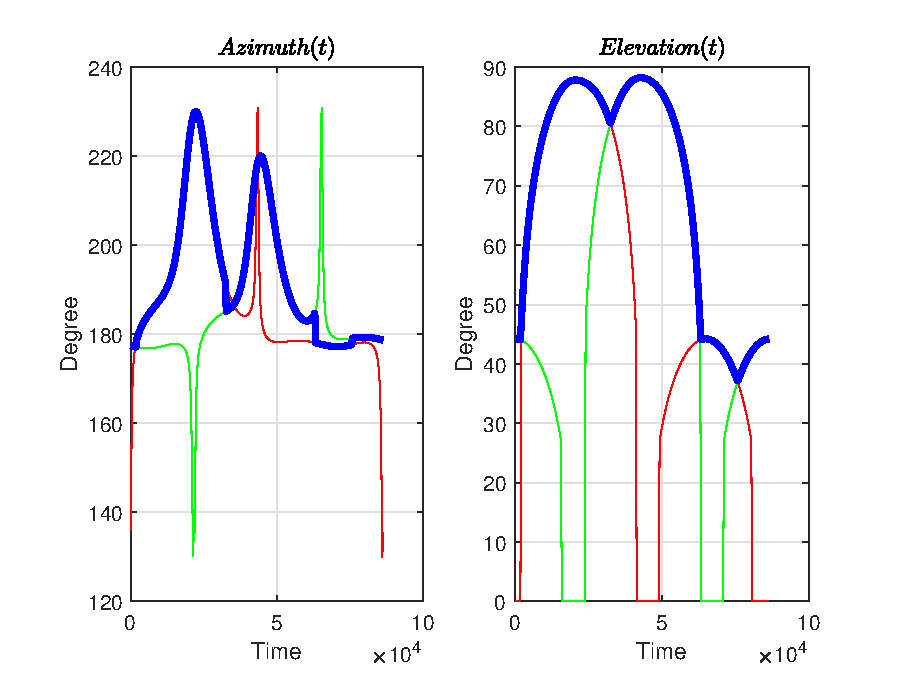
\includegraphics[width=.5\textwidth]{EL_AZ_GS.eps}
		\caption{Elevation and Azimuth in the Ground Station Position}
		\label{fig:elevation_final}
	\end{figure}
\subsection{Ground Station requirements}
	The requirements for the \gls{gs} are substantially the following:
	\begin{itemize}
		\item the Internet connection;
		\item the antenna model and specifications.
	\end{itemize}

	The Internet connection is the most important (if not the only one) reason for the existence of the \gls{gs}, since one of 			the problem requirements is indeed the possibility of video calls and other internet services.

	For the antenna model we chose a reflector antenna with a single circular beam; the antenna parameters are listed in \autoref{tab:antennaParam}.
	\begin{table}
		\centering
		\begin{tabular}{lr}
		\toprule
		Parameter & Value\\
		\midrule
		Frequency Band & Ku Band\\
		Dish diameter D & 6 m\\
		Efficiency & 0.6\\
		\bottomrule
		\end{tabular}
		\caption{\gls{gs} antenna specifications}
		\label{tab:antennaParam}
	\end{table}

	Another aspect to consider is the fact that the variations in the azimuth values are very steep in a specific moment of the satellite revolution, and this brings as side effect the temporary suspension of the service for the time needed by the \gls{gs} to point properly the correct satellite in orbit (about 2 minutes).
	To avoid this problem, two antennas in the \gls{gs} can be used.
\subsection{User requirements}
The user requirements are substantially the model of the antenna and the dimension of the dish: the model is identical to the ones used for the satellite and the \gls{gs}, so a reflector antenna with a single beam; the dish diameter is smaller in this case, for a matter of space and feasibility, and is of 1 m. There is no need, in this case, of specifying the position of the users since by definition they are mobile users. As example we put the user in 71N,45E, that corresponds to a rain rate $R = 4.5554 mm/h$.
